%
% !BIB TS-program = biber
% !BIB program = biber
% !TeX spellcheck = en_US
% !TeX program = lualatex
%
% support document for version: v 3.00  Feb 2026   Volker RW Schaa
%   
%
\documentclass[%              % paper size definition not needed as JACoW page size is set
               %boxit,        % show page boundaries to check whether paper is inside correct margins
               %refpage       % references placed on separate page
               %biblatex,     % BibLaTeX is to be used
               %nospread,     % flushend option: do not fill with whitespace to balance columns
               %hyphens,      % allow \url to hyphenate at "-" (hyphens)
               %luatex,       % use LuaLaTeX to process the file
               ]{jacow}

\usepackage[english]{babel}
\usepackage{physics}

\listfiles

%%
%% Lengths for the spaces in the title
%%   \setlength\titleblockstartskip{..}  %before title, default 3pt
%%   \setlength\titleblockmiddleskip{..} %between title + author, default 1em
%%   \setlength\titleblockendskip{..}    %afterauthor, default 1em

\begin{document}

%%%%% Title - Author block generated from indico contribution details %%%%%
%%%%%%%%%%%%%%%%%%%% Do not modify  %%%%%%%%%%%%%%%%%%%%%%%%%
%%%%% If you need to modify the content of this block, do it by modifying the  %%%%%
% \title{MODELING AND CORRECTION OF SIRIUS STORAGE RING NONLINEAR OPTICS}
% \title{Assessment of Sextupole Strength Identifiability in NOECO Calibration at SIRIUS}
% \title{Assessment of NOECO for Nonlinear Optics Calibration at the SIRIUS Storage Ring}
\title{Application of the Nonlinear optics from off-energy orbits method at the SIRIUS Storage Ring}


\author{M.~Velloso\thanks{matheus.velloso@lnls.br}\textsuperscript{1}, L.~Liu, X.~Resende, F.~H.~de Sá, Brazilian Synchrotron Light Laboratory, Campinas, Brazil\\
\textsuperscript{1}also at Gleb Wataghin Institute of Physics, University of Campinas, Campinas, Brazil
}

\maketitle

%%%%% End of Title - Author block %%%%%

%%%%% You can modify the abstract to add LaTeX commands. However, please make sure that it is similar to the one in indico %%%%%
\begin{abstract}
 % Attempts at nonlinear optics calibration at SIRIUS storage ring using the Nonlinear Optics from Closed Orbits (NOECO) method are presented.  The NOECO fitting setup adapted for SIRIUS is summarized and the acquisition of off-energy orbit response matrices (OEORMs) at the storage ring is described. Analysis of SIRIUS case  highlights the presence of quasi-degeneracies that can limit sextupole strengths identifiability.
 The applicability of the Nonlinear Optics from Off-Energy Closed Orbits (NOECO) method to the SIRIUS storage ring is investigated. Off-energy orbit response matrices (OEORMs) were measured and used for sextupole strength calibration through a Levenberg-Marquardt (LM) fitting procedure with Tikhonov regularization. The fitted strengths reproduced the measured chromaticities with reasonable accuracy and were consistent with control system estimates. Analysis of the OEORM Jacobian revealed strong correlations among sextupole family signatures, indicating significant quasi-degeneracies in the inverse problem. Machine experiments and model-based simulations showed that localized perturbations are redistributed across correlated families, especially in the presence of small optics mismatches. The results indicate that OEORM-based calibration is feasible at SIRIUS, although its resolving power is fundamentally limited by parameter correlations and model imperfections.
\end{abstract}

\section{Introduction}
NOECO~\cite{olsson_nonlinear_2020} is a calibration method that fits chromatic sextupole strengths to best reproduce the measured OEORM, in a least-squares sense.
The OEORM is defined as the numerical derivative of the orbit response matrix (ORM) with respect to relative energy deviations $\delta$:
\begin{equation}
\text{OEORM} = \frac{\text{ORM}_{+\delta} - \text{ORM}_{-\delta}}{2 \delta},
\label{eq:oeorm_def}
\end{equation}
where $\text{ORM}_{\pm \delta}$ corresponds to the ORM measured at energy deviation $\pm\delta$ and ORM elements read
\begin{equation}
    \text{ORM}_{ij} = \frac{\Delta u_i}{\Delta \theta_j},
\end{equation}
with $\vb{u} = \mqty[\vb{x} & \vb{y}]^\intercal$ and $\Delta \boldsymbol{\theta} = \mqty[\boldsymbol{\theta}_x & \boldsymbol{\theta}_x]^\intercal$. 
At SIRIUS, like the ORM, the OEORM is a $320 \times 281$ matrix, with the dispersive orbit response as the last column.
% where the 160 top/bottom rows correspond to horizontal/vertical BPMs and the 281 columns correspond to the orbit signatures of the 120 horizontal correctors (CH), 160 vertical correctors (CV) and 1 RF (dispersion) column. 
% Figure~\ref{fig:oeorm_cols} shows
% two particular columns from the OEORM diagonal blocks\footnote{i.e. the horizontal/vertical BPMs signatures due to the horiztonal/vertical steerers.}, calculated at SIRIUS model.

% \begin{figure}
%     \centering
%     \includegraphics[width=\linewidth]{oeorm_col.pdf}
%     \caption{Two columns from SIRIUS model OEORM diagonal blocks: horizontal BPMs readings along horizontal CM column (blue), and vertical BPMs readings along vertical CV column (red). Measurement simulated with $\delta=0.5\%$ in a LOCO-calibrated model.}
%     \label{fig:oeorm_cols}
% \end{figure}

% \begin{figure*}[!htb]
%     \centering
%     \includegraphics*[width=0.95\textwidth]{oeorm_col_diff.pdf}
%     \caption{Deviations in two OEORM diagonal-block columns (horizontal on the left, vertical on the right) relative to the OEORM at operational strengths. Each curve corresponds to a distinct strength perturbation applied to the SDP2 sextupole family.}
%     \label{fig:col_diff}
% \end{figure*}
% The SIRIUS storage ring consists on a 20-cell five-bend-achromat (5BA) lattice comprising a 5-fold symmetric configuration with alternating high- and low- horizontal betatron functions.
%A superperiod consists of one high-beta and 3 low-beta sections arranged as A-B-P-B. 
%The B and P low-beta sections have identical first order optics, but their sextupoles are different. 
Regarding SIRIUS sxtupole lattice, there are 6 achromatic sextupole families in the straight sections
% SFA0, SDA0, SFB0, SDB0, SDP0, SFP0 
and 15 chromatic families in the arcs.
%SDA1, SFA1, SDA2, SFA2, SDA3, SDB1, SFB1, SDB2, SFB2, SDB3, SFP1, SDP1, SFP2, SDP2, SDP3. 
The NOECO scheme purports to calibrate the chromatic lattice only.

\section{OEORM measurements at SIRIUS}

OEORM measurements at the SIRIUS storage ring are carried out according to the following procedure. Energy deviations of $\delta=\pm 0.5 \times 10^{-2}, \pm 0.25 \times 10^{-2}$ are introduced into the beam by adjusting the RF master oscillator frequency around the nominal operating frequency $f_0$. The required frequency shifts $\Delta f$ are calculated as $\Delta f = -\alpha f_0 \delta$, where $\delta$ is the desired energy shift and $\alpha = 1.636\times10^{-4}$ is the lattice momentum compaction factor at $\delta=0$.

At each energy offset, a fast ORM measurement (``AC'' measurement) \cite{velloso:ipac2022-mopotk002} is performed. Using the ORMs measured over the energy shift range together with the ORM at $\delta=0$, the data are fitted with a linear model of ORM versus energy deviation. The OEORM corresponds to the angular coefficient of the fit.

\section{The fitting setup}
%NOECO aims to match model and machine OEORMs in a least-squares sense.
The objective function to be minimized is
\begin{equation}
\chi^{2} = \sum\limits_{ij}\frac{|\text{OEORM}_{ij}^{\text{meas}} - \text{OEORM}_{ij}^{\text{model}}|^2}{w^2_{ij}},
\end{equation}
where $\text{OEORM}^{\text{meas}}$ is the measured OEORM and $\text{OEORM}^{\text{model}}$ the model prediction. The weights $w_{ij}$ represent the OEORM experimental noise, 
% as propagated from eq.~\eqref{eq:oeorm_def}:
% $w_{ij} = \frac{\sigma_{i}}{\theta_j\delta}$;
% with $\sigma_i$ being the noise of the $i$-th BPM and $\theta_j$ the kick amplitude of the $j$-th steerer. 
% The BPM noise is given by $\sigma_i = \sum_j \sigma_{ij}$, where $\sigma_{ij}$ is the noise at the $i$-th BPM at the $j$-th corrector frequency, which is estimated by fitting the amplitude $a_{ij}$ in a non-perturbed orbit acquisition.
% With this weighting, $\chi^2$ is dimensionless. 
% If the model and the experimental noise are representative, when parameters are well tuned, $\chi^2/N \sim 1$, where $N$ is the number of OEORM entries being fitted\footnote{Strictly, $\chi^2/\text{dof}\sim 1$, where $\text{dof}=N - N_p$. We use $N$ because, $N=44960$, $N_p=615$, so $N\gg N_p$.}.
%\subsection{Calibration parameters}

The fitting parameters are the chromatic sextupole strengths (15 knobs) together with calibration gains for BPM readings (320) and calibration gains for corrector strengths (280). The gains enter the minimization as linear transformations applied to the measured OEORM:
\begin{equation}
    \text{OEORM}^{\prime\text{meas}} =  G^\text{BPM}~\text{OEORM}^{\text{meas}}~G^{\text{corr}}.
\end{equation}
% where
% \begin{equation}
% T = {G}^{\text{BPM}} + C
% \end{equation}
% \begin{equation}
%  G^\text{BPM} = \text{diag}(g_{0}^\text{BPM}, \dots, g_{159}^{\text{BPM}}, \dots, g_{319}^{\text{BPM}})
% \end{equation}
% \begin{equation}
%  G^\text{corr} = \text{diag}(g_{0}^\text{corr}, \dots, g_{119}^\text{corr}, g_{120}^\text{corr}, \dots, g_{279}^{\text{corr}})
% \end{equation}
% \begin{equation}
%     C = \mqty[{0} & {C}_{x}\\ {C}_{y} & {0}]
% \end{equation} 
% \begin{equation}
%     {C}_{x} = \text{diag}(c_{0}, \dots, c_{159}), \quad  {C}_{y} = \text{diag}(c_{160}, \dots, c_{319})
% \end{equation} 
The parameter vector to be calibrated is organized as
% $$\vb{P} = \mqty[\vb{S} & \vb{G}^{\text{corr}} & \vb{G}^{\text{BPM}} & \vb{C}]^\intercal$$
$$\vb{P} = \mqty[\vb{S} & \vb{G}^{\text{corr}} & \vb{G}^{\text{BPM}}]^\intercal,$$
% with dimensions $15 + 280 + (2\times 160) + (2\times 160) =  935$. If coupling are excluded, as discussed below, then the dimensions are reduced to $615$.
with dimensions $15 + (120 + 160) + (2\times 160) =  615$. 
% The theoretical dependence of OEORM entries on sextupole knobs applies only to the matrix diagonal blocks.
Off-diagonal elements of the OEORM are not considered in the fitting, eliminating the need of couplings among the horizontal and vertical BPMs signals as additional parameters. 
% gains obtained from a previous LOCO fitting can be used, reducing the free parameters to the chromatic sextupole lattice only.
%Our best results were attained in this manner, so we focus on sextupoles fitting from now on.

% \begin{figure*}[!h]
%     \centering
%     \includegraphics*[width=0.95\textwidth]{jacobian_svd_modes.pdf}
%     \caption{Jacobian singular values spectrum, on the left. Components of the lowest singular value modes, on the right.}
%     \label{fig:svd}
% \end{figure*}
%\subsection{Parameters updates}
The vector $\vb{P}$ minimizing the least-squares problem is iteratively calculated until convergence as $\vb{P}^{(n+1)}\to \vb{P}^{(n)} + \Delta \vb{P}^{(n)}$, with Levenberg-Macquardt (LM) steps 
\begin{equation}
\Delta \vb{P}^{(n)} = - \left[J^{\intercal}J  + \lambda \text{diag}(J^{\intercal}J) \right]^{-1} J^\intercal \vb{r}^{(n-1)},
\label{eq:GN}
\end{equation}
with $\vb{r}^{(n)}$ being the residuals vector at the $n$-th iteration. The residuals elements $r_k = \left(\vb{r}^{(n)}\right)_k$ are obtained from the vectorization of the weighted OEORM residue ath the $n$-th iteration
    \begin{equation}
    r_{k} = \frac{\text{OEORM}_{ij}^{\prime\text{meas}}- \text{OEORM}_{ij}^{\text{model}}}{w_{ij  }},
    \end{equation}
with $\quad k = 281 i + j, \quad 0\leq i\leq 319, \quad 0\leq j\leq 280$, 
and $J$ is the Jacobian matrix: 
\begin{equation}
J_{kl} = \pdv{r_k}{P_l}.
\end{equation}
% In terms of the residual vector, the objective function reads $\chi^2 = \vb{r}^\intercal \vb{r}$. 
The Jacobian columns corresponding to the sextupole knobs are calculated numerically with OEORM measurement simulations in the model. The columns corresponding to correctors and BPMs gains can be calculated analytically.
% With the inclusion of Levenberg-Macquardt (LM) and L2 regularizations, equation \eqref{eq:GN} reads
% \begin{equation}
% \Delta \vb{P}^{(k)} = - \left[J^{\intercal}J + \lambda \text{diag}(J^{\intercal}J) + \text{diag}(\boldsymbol{\alpha}^\intercal\boldsymbol{\alpha})\right]^{+} J^\intercal \vb{r}^{(k)},
% \end{equation}
% The $\boldsymbol{\alpha}$ vector has entries $\alpha_i$ corresponding to a penalty to the $i$th fitting parameter. We restrict ourselves to fixing $\alpha_i=\alpha$, for the sextupole stregths, i.e. $i=0, \dots, 14$, and zero to the other parameters. In this manner we are penalizing large excursions in the sextupole strengths. Determination of hyperparameters $\lambda$ and $\alpha$ will be discussed in the next section.

% \subsection{OEORM block selection}
% The OEORM is a $320\times281$ matrix. When vectorized with all blocks included, it yields a vector of $89920$ entries. However, the theoretical dependence of OEORM entries on sextupole knobs applies only to the diagonal blocks; off-diagonal terms are higher-order effects. In our measurements, these off-diagonal entries are orders of magnitude smaller, confirming that the OEORM is effectively block-diagonal. For this reason, only the diagonal blocks are used in the fit, and only the horizontal-dispersion column is retained. The resulting fitting vector has dimension $44960$. With only diagonal blocks included, coupling coefficients between BPM planes need not be fitted. The remaining parameters, beyond the sextupole strengths, are the steerer and BPM gains, totaling $615$ parameters. The Jacobian, thus, is a $44960\times615$ matrix.

%\subsection{Regularizations}
The LM constant $\lambda$ is updated adaptively depending on whether $\chi^2$ improves or worsens. Additional Tikhonov/Ridge regularization of the form $\chi^2 \to \chi^2 + \|W^\intercal \Delta \vb{P}\|^2$, with $W = \alpha I_{15}$, is applied to mitigate degeneracies and prevent excessive excursions of the sextupole strengths.
With the regularization, the normal equation reads $\Delta \vb{P}^{(n)} = - A^{-1} J^\intercal \vb{r}^{(n-1)}$, where matrix $A$ reads
\begin{equation}
A =  J^{\intercal}J  + \lambda \text{diag}(J^{\intercal}J) + W^\intercal W.
\label{eq:normal_mat}
\end{equation}
\begin{figure}[!]
    \centering
    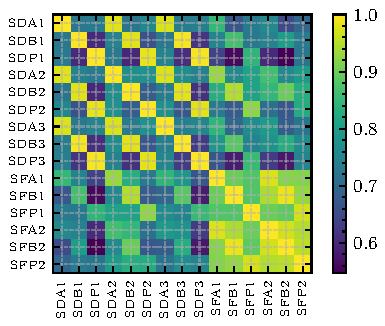
\includegraphics[width=0.9\linewidth]{THP5303_f1.pdf}
    \caption{Jacobian columns pairwise correlation, or cosine distance. Columns are highly correlated, meaning many sextupole families display similar OEORM signatures.} 
    \label{fig:jac_corr}
\end{figure}

\section{Degeneracies and parameters selection}

The pairwise correlations between Jacobian columns $i$ and $j$, defined as $C_{ij} = \frac{J_i \cdot J_j}{\norm{J_i}\norm{J_j}}$ and shown in Fig.~\ref{fig:jac_corr}, highlight strong collinearities among the family signatures, particularly within a highly correlated cluster formed by the focusing sextupole families. This indicates that several knobs produce similar signatures in the off-energy orbit responses, limiting the identifiability of individual knobs and potentially leading to an ill-posed optimization problem. 

The singular value decomposition of the matrix $A$ from Eq.~\eqref{eq:normal_mat} reveals a condition number of $10^{6}$, which can be improved through an appropriate choice of the LM parameter $\lambda$ and the Tikhonov regularization parameter $\alpha$. In our tests, the values $\lambda=10^{-3}$ and $\alpha=10^{2}$ raised the singular value spectrum, improved the conditioning, attenuated degeneracies and still provided an acceptable convergence time of approximately 10 iterations.

\section{Fitting results}
\subsection{Error identification in the machine}
% NOECOs ability to fit the nonlinear lattice strengths and reveal deliberately introduced perturbations to a given family strength was tested in the machine model. The OEORM  was calculated for the nominal lattice with a 2\% perturbation on a given family strength. Synthetic noise was added to simulate BPMs reading errors. The LM parameter \(\lambda\) was initialized at \(1\times10^{-3}\) and updated by a factor of 10 each iteration, depending on whether \(\chi^2\) improved or worsened. A fixed Tikhonov regularization of $\alpha=10^{2}$ was applied to sextupole knobs. NOECO correctly identified the point perturbation up to a X precision. 
Our initial test of the NOECO scheme consisted on benchmarking the method's ability to identify intentionally introduced perturbations. Three OEORMs were measured under three sextupoles strength configurations. The first corresponds to the current operational strengths, defined in 2023 through online optimization of injection efficiency and dynamic aperture~\cite{vellosomatheus_online_2023}. The other two measurements use the same operational settings with additional point perturbations of \(+1\%\) and \(+2\%\) applied to the SDP2 sextupole family. We denote these measurements as OEORM0 (operational), OEORM1 (1\% perturbation), and OEORM2 (2\% perturbation). An ORM measurement at operation strengths sextupoles and nominal energy is used to fit a LOCO model which in turn was used both to calculate the NOECO Jacobian and to perform all OEORM measurement simulations. The NOECO fit free parameters consisted solely of the sextupole family strengths, since BPM and steerer gains were not included in the fit and their values obtained from the LOCO model were used instead. The LM parameter \(\lambda\) was initialized at \(10^{-3}\) and updated by a factor of 10 each iteration, depending on whether \(\chi^2\) improved or worsened. A fixed Tikhonov regularization of $\alpha=10^{2}$ was applied to sextupole knobs.
% and a singular-value cutoff was applied, excluding modes with \(s_i/s_{\text{max}} < 1\times10^{-4}\) from the pseudo-inverse to handle the dominant BPM/steerer degeneracy. All calibrations used a fixed Jacobian computed from a LOCO-calibrated model with nominal sextupole strengths. Jacobian computation for the SIRIUS model using the pyaccel and trackcpp tracking libraries takes about 2.5 minutes.

\begin{figure*}[!h]
    \centering
    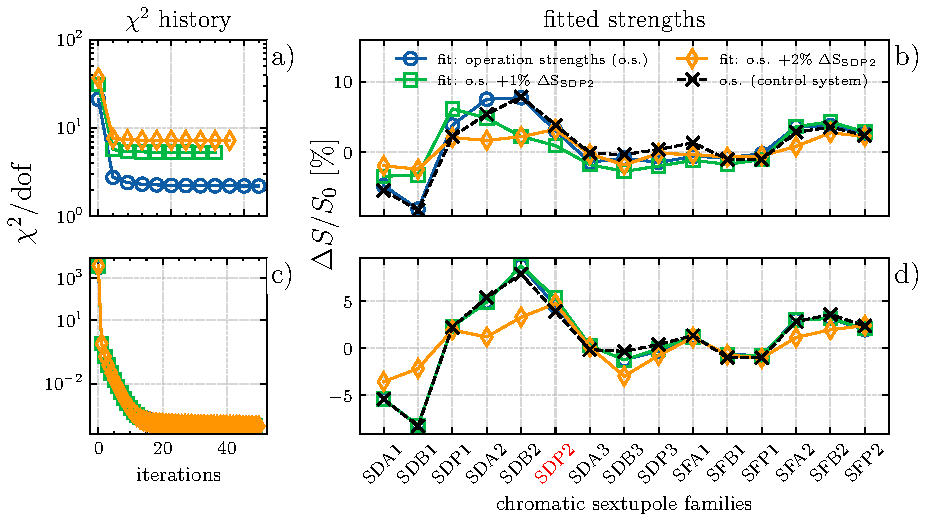
\includegraphics[width=\linewidth]{THP5303_f2.pdf}
    \caption{History of objective function throughout the optimization (left) and relative variations with respect to nominal model strengths required to explain measured OEORMs (right). Black curve corresponds to control system sextupole strengths.} 
    \label{fig:fit_strengths}
\end{figure*}


% We refer to this as a non-sequential fitting scheme, in contrast to a sequential approach in which OEORM0 is fitted from nominal parameters, OEORM1 is fitted starting from the OEORM0 solution, and OEORM2 from the OEORM1 solution. Tests using both schemes produced identical results, so only the non-sequential case is reported here. 
Figure~\ref{fig:fit_strengths} shows, on the left, the evolution of \(\chi^2/\text{dof}\) for each measured OEORM, while, on the right, the resulting fitted strengths are shown as relative variations with respect to the model nominal strengths. The blue curves correspond to the fit to the operation strengths, whereas the green and orange curves correspond to the 1\% and 2\% perturbations, respectively. The black curve represents the control system strength readings, which are strength estimates from the magnet excitation curves and the design beam energy.

Although \(\chi^2/\text{dof}\) decreases throughout the minimization, its final value for OEORMs 1 and 2 remains above unity, as values close to one would be expected for a representative model and weithing $w_{ij}$. This may indicate incomplete modeling.

The strengths fitted to the operation strengths resemble the control system estimates and yield model chromaticities \((\xi_x, \xi_y) = (3.17, 2.91)\), in reasonable agreement with the measured values of \((3.11, 2.67)\). Without machine measurements of nonlinear-optics functions, however, it is difficult to assess whether the model with NOECO-fitted strengths also reproduce the machine’s nonlinear optics, which would serve as an additional validation of the calibration. The method's ability to fit the nonlinear optics and provide a representative nonlinear lattice model can still be validated with iterative correction or symmetrization, which is an upcoming effort.

Regarding the introduced perturbations, NOECO was not able isolate them within the SDP2 family alone, highlighting the issues with identifiability anticipated by the analysis of the Jacobian columns co-linearities. 
\subsection{Error identification in the model}
Given the method's difficulty in identifying isolated perturbations, model-based simulations were carried out to assess the extent to which identifiability is feasible. In the tests, when a given machine model is perturbed solely in the sextupole lattice, the NOECO fitting is able to reproduce the perturbed strengths, both for isolated perturbations and for distributed perturbations across all families. However, if additional optics mismatches are present, the correct identification of perturbations is no longer guaranteed. A small perturbation of 0.3\% in a single chromatic quadrupole, introducing a slight tune variation at the third decimal place and a sub-1\% beta-beating, is already sufficient to limit the identifiability of isolated perturbations. This is a typical magnitude of quadrupole gradient variation that is usually left uncorrected in the machine during LOCO optics symmetrization.

These conclusions were drawn from the following simulations. The nominal model is duplicated, and a small quadrupole variation is introduced together with the nonlinear lattice perturbations that are intended to be identified. The OEORM is then calculated for this perturbed model and used as the target OEORM to be reproduced. The nominal, unperturbed model used internally by NOECO to calculate the OEORM of candidate strengths and the Jacobian has its tunes and chromaticities corrected to match those of the perturbed model being fitted. The fit is then performed using the same hyperparameters adopted in the machine OEORM fits.

We speculate that, due to the strong co-linearities among the OEORM signatures, even slight optics mismatches introduce additional OEORM components that cannot be fully represented by the nominal model. These incompatible signatures may then be projected onto particular strength signatures within highly correlated families that can partially reproduce the observed OEORM variation. Since small optics mismatches between the machine and the model are unavoidable, the ability of NOECO to identify isolated perturbations in the SIRIUS case appears to be fundamentally limited.

\section{Conclusions}
An initial assessment of NOECO's applicability to the SIRIUS storage ring has been presented. The calibration method was applied both to fit the machine operational strengths and to benchmark its ability to identify intentionally introduced errors. The strengths fitted to the operational OEORM reproduced the machine chromaticities with reasonable accuracy and showed good agreement with the strength estimates from the control system. The representativeness of the fitted strengths can be further validated by verifying whether iterative nonlinear optics symmetrizations in the machine converge.

When perturbations were introduced into the operational strengths, NOECO redistributed them across correlated families rather than identifying them individually. Identifiability is also limited in model-based simulations, especially in the presence of optics mismatches. This reflects the quasi-degeneracy intrinsic to the machine sextupole, corrector, and BPM layout, as highlighted by the strong correlations in the SIRIUS OEORM Jacobian. 

Overall, the results indicate that OEORM-based calibration may be feasible at SIRIUS, but its resolving power is fundamentally limited by strong parameter correlations. Mitigating these limitations may require the inclusion of additional observables capable of breaking the degeneracies, or the use of different observables altogether.


%\begin{thebibliography}{99}   	% Use for  10-99  references

\begin{thebibliography}{9}

    \bibitem{olsson_nonlinear_2020}
    D. K. Olsson, Å. Andersson, M. Sjöström,
    \textquotedblleft{Nonlinear optics from off-energy closed orbits}\textquotedblright,
    \emph{Physical Review Accelerators and Beams}, vol. 23, p. 102803, 2020.
    \url{doi:10.1103/PhysRevAccelBeams.23.102803}
    
    \bibitem{PhysRevAccelBeams.26.032803}
    D. Vilsmeier, R. Singh, M. Bai,
    \textquotedblleft{Inverse modeling of circular lattices via orbit response measurements in the presence of degeneracy}\textquotedblright,
    \emph{Phys. Rev. Accel. Beams}, vol. 26, p. 032803, Mar. 2023.
    \url{doi:10.1103/PhysRevAccelBeams.26.032803}

    %\cite{velloso:ipac2022-mopotk002}
    \bibitem{velloso:ipac2022-mopotk002}
    M. M. S. Velloso, M. B. Alves, and F. H. de Sá,
    \textquotedblleft{Fast Orbit Response Matrix Measurement via Sine-Wave Excitation of Correctors at Sirius}\textquotedblright,
    % --- abbreviated form (published paper) - JACoW template Feb 2018 ---
    in \emph{Proc. IPAC'22}, Bangkok, Thailand, Jun. 2022, pp. 425--428.
    % --- complete form (published paper) - JACoW template Feb 2018 ---
    %  in \emph{Proc. 13th International Particle Accelerator Conference (IPAC'22)}, Bangkok, Thailand, Jun. 2022, pp. 425--428.
    \url{doi:10.18429/JACoW-IPAC2022-MOPOTK002}
    % --- additional material -ISSN/ISBN--
    %  ISBN: 978-3-95450-227-1, ISSN: 2673-5490

    
    \bibitem{huang2019beam}
    X. Huang,
    \textquotedblleft{Beam-based Correction and Optimization for Accelerators}\textquotedblright,
    CRC Press, 2019.
    ISBN: 9780429784743.
    
    \bibitem{vellosomatheus_online_2023}
    M.~M.~S.~Velloso,  M.~B.~Alves, L.~Liu, X.~Huang, X.~R.~Resende and F.~H.~de~Sá,
    \textquotedblleft{Online optimization of SIRIUS nonlinear optics}\textquotedblright,
    in \emph{Proc. IPAC’23}, sep. 2023, pp. 3302--3305.
    \url{doi:10.18429/JACOW-IPAC2023-WEPL087}
    
\end{thebibliography}


\end{document}